\chapter{原子内部}\label{ch:g9:inside-the-atom}

1909 年，在曼彻斯特的一间实验室里，一束微小而快速的粒子
被射向一片仅有几百个\omterm{def:g7:atoms-and-molecules:atom}{原子}厚的金箔。几乎所有粒子
都径直穿过，仿佛金箔是空的。但大约每几千个粒子中，
就有一个被弹了回来。“这就像你用 15 英寸炮弹射向一张薄纸，
结果它竟弹回来击中了你，”卢瑟福说，做实验的是他的学生。\omterm{def:g7:atoms-and-molecules:atom}{原子}，
这种不可分割的物质单元，
竟有着内部结构——
而且几乎是完全空的。

\begin{recall}
所有物质都由\omterm{def:g7:atoms-and-molecules:atom}{原子}组成，\omterm{def:g7:atoms-and-molecules:atom}{原子}大约有一百种，
每种\omterm{def:g7:atoms-and-molecules:atom}{原子}都有一个符号，如 \ce{H}、\ce{C}、\ce{O}、\ce{Fe}。\omterm{def:g7:atoms-and-molecules:atom}{原子}
可结合成\omterm{def:g7:atoms-and-molecules:molecule}{分子}，\omterm{def:g7:atoms-and-molecules:molecule}{分子}可用化学式表示，例如 \ce{H2O}
（见\cref{ch:g7:atoms-and-molecules}）。
\end{recall}

\section{原子核与电子}

\begin{definition}[原子核与电子]\label{def:g9:inside-the-atom:nucleus}
每个\omterm{def:g7:atoms-and-molecules:atom}{原子}都有一个微小、致密的核心，即\emph{原子核}\index{原子核}，
它带正电荷。绕其运动的是质量轻得多的
粒子，即\emph{电子}\index{电子}，每个电子都带有相同的
负电荷 $-e$。
\end{definition}

\begin{proposition}[原子呈电中性]\label{prop:g9:inside-the-atom:neutral}
% ledger: const:e
整个\omterm{def:g7:atoms-and-molecules:atom}{原子}不带电：其\omterm{def:g9:inside-the-atom:nucleus}{原子核}所带的正电荷
恰好与其\omterm{def:g9:inside-the-atom:nucleus}{电子}所带的负电荷相互抵消。
电荷 $e$ 很小：$e = \qty{1.60e-19}{C}$（库仑，
即电荷的单位，参见 One Physics Book）。
\end{proposition}

\begin{omfigure}
\begin{tikzpicture}[font=\small]
  \shade[inner color=omDef!35, outer color=white] (0,0) circle (2.2);
  \draw[omDef!60, dashed] (0,0) circle (2.2);
  \foreach \a/\r in {20/1.6,95/1.1,150/1.9,215/1.4,290/1.7,340/0.9} {
    \fill[omDef] (\a:\r) circle (0.06);
    \node[font=\scriptsize, omDef] at ($(\a:\r)+(0.18,0.16)$) {$-$};
  }
  \fill[red!70!black] (0,0) circle (0.1);
  \draw[<-, omProp, thick] (-0.12,0.02) -- (-3.0,0.9) node[left, text=black, align=right]
    {原子核：微小、\\ 致密、带正电};
  \draw[<-, omProp, thick] ($(20:1.6)+(0.08,0.02)$) -- (3.0,0.9) node[right, text=black]
    {电子：质量小、带负电};
  \draw[<-, omProp, thick] (300:2.2) -- (3.0,-1.4) node[right, text=black, align=left]
    {电子在原子核周围的 \\ 电子云中运动};
\end{tikzpicture}

{\small \omterm{def:g7:atoms-and-molecules:atom}{原子}示意图，未按比例绘制。若将\omterm{def:g9:inside-the-atom:nucleus}{原子核}画成与红点一样大，
则\omterm{def:g9:inside-the-atom:nucleus}{电子}云的直径约为几百米。}
\end{omfigure}

\section{质子与中子}

\begin{definition}[质子、中子与核子]\label{def:g9:inside-the-atom:proton}
\omterm{def:g9:inside-the-atom:nucleus}{原子核}由两种粒子组成：\emph{质子}\index{质子}，
每个质子带电荷 $+e$，\emph{中子}\index{中子}
不带电。质子与中子的质量几乎相同，
二者合称为\emph{核子}\index{核子}。
\end{definition}

\begin{definition}[原子序数与质量数]\label{def:g9:inside-the-atom:atomic-number}
\omterm{def:g9:inside-the-atom:nucleus}{原子核}中的\omterm{def:g9:inside-the-atom:proton}{质子}数称为\emph{原子序数}\index{原子序数}，
记作 $Z$。\omterm{def:g9:inside-the-atom:proton}{核子}的数目
（\omterm{def:g9:inside-the-atom:proton}{质子}与\omterm{def:g9:inside-the-atom:proton}{中子}合计）称为\emph{质量数}\index{质量数}，
记作 $A$。\omterm{def:g9:inside-the-atom:proton}{中子}数为 $N = A - Z$。
\end{definition}

\begin{notation}[核素符号]\label{not:g9:inside-the-atom:symbol}
具有给定\omterm{def:g9:inside-the-atom:nucleus}{原子核}的\omterm{def:g7:atoms-and-molecules:atom}{原子}，用其符号表示，左上角为\omterm{def:g9:inside-the-atom:atomic-number}{质量数}，
左下角为\omterm{def:g9:inside-the-atom:atomic-number}{原子序数}：
\ce{^{A}_{Z}X}。例如 \ce{^{12}_{6}C} 有 6 个\omterm{def:g9:inside-the-atom:proton}{质子}，$12 - 6 =
6$ 个\omterm{def:g9:inside-the-atom:proton}{中子}；\ce{^{56}_{26}Fe} 有 26 个\omterm{def:g9:inside-the-atom:proton}{质子}和 30 个\omterm{def:g9:inside-the-atom:proton}{中子}。
\end{notation}

\begin{method}[读取核素符号]\label{met:g9:inside-the-atom:read}
对于 \ce{^{A}_{Z}X}：
\begin{enumerate}
  \item \omterm{def:g9:inside-the-atom:proton}{质子}数：$Z$；
  \item \omterm{def:g9:inside-the-atom:proton}{中子}数：$A - Z$；
  \item 电中性\omterm{def:g7:atoms-and-molecules:atom}{原子}的\omterm{def:g9:inside-the-atom:nucleus}{电子}数：$Z$，与\omterm{def:g9:inside-the-atom:proton}{质子}数相同。
\end{enumerate}
\ce{^{23}_{11}Na} 有 11 个\omterm{def:g9:inside-the-atom:proton}{质子}、12 个\omterm{def:g9:inside-the-atom:proton}{中子}和 11 个\omterm{def:g9:inside-the-atom:nucleus}{电子}。
\end{method}

\begin{omfigure}
\begin{tikzpicture}[font=\small]
  \node[font=\Huge, inner sep=1pt] (x) at (0,0) {\ce{^{35}_{17}Cl}};
  \draw[<-, omProp, thick, shorten <=3pt] ([xshift=5pt,yshift=-7pt]x.north west) -- (-2.6,1.0)
    node[left, text=black, align=right] {质量数 $A = 35$：\\ 质子数 + 中子数};
  \draw[<-, omProp, thick, shorten <=3pt] ([xshift=5pt,yshift=7pt]x.south west) -- (-2.6,-1.0)
    node[left, text=black, align=right] {原子序数 $Z = 17$：\\ 质子数};
  \draw[<-, omProp, thick] ([xshift=2pt]x.east) -- (2.2,0) node[right, text=black,
    align=left] {元素符号：\\ 氯};
\end{tikzpicture}

{\small 读取核素符号：这种氯\omterm{def:g7:atoms-and-molecules:atom}{原子}有 17 个\omterm{def:g9:inside-the-atom:proton}{质子}，
$35 - 17 = 18$ 个\omterm{def:g9:inside-the-atom:proton}{中子}，电中性时有 17 个\omterm{def:g9:inside-the-atom:nucleus}{电子}。}
\end{omfigure}

\section{元素与同位素}

\begin{definition}[元素]\label{def:g9:inside-the-atom:element}
\emph{元素}\index{元素}是指所有
\omterm{def:g9:inside-the-atom:atomic-number}{原子序数} $Z$ 相同的\omterm{def:g7:atoms-and-molecules:atom}{原子}，以及由它们形成的带电\omterm{def:g7:atoms-and-molecules:atom}{原子}的集合。
每种元素都有名称和符号：凡\omterm{def:g9:inside-the-atom:proton}{质子}数为 6 的\omterm{def:g7:atoms-and-molecules:atom}{原子}，
都是碳\omterm{def:g7:atoms-and-molecules:atom}{原子}，\ce{C}；凡\omterm{def:g9:inside-the-atom:proton}{质子}数为 8 的\omterm{def:g7:atoms-and-molecules:atom}{原子}，
都是氧\omterm{def:g7:atoms-and-molecules:atom}{原子}，\ce{O}。
\end{definition}

\begin{definition}[同位素]\label{def:g9:inside-the-atom:isotope}
同一\omterm{def:g9:inside-the-atom:element}{元素}中，\omterm{def:g9:inside-the-atom:proton}{中子}数不同的\omterm{def:g7:atoms-and-molecules:atom}{原子}，
因而\omterm{def:g9:inside-the-atom:atomic-number}{质量数}也不同，互为该\omterm{def:g9:inside-the-atom:element}{元素}的\emph{同位素}\index{同位素}。
它们的 $Z$ 相同，而 $A$ 不同。
\end{definition}

\begin{example}[碳和氢的同位素]\label{ex:g9:inside-the-atom:isotopes}
% ledger: iso:C12, iso:C13, iso:H2
天然碳中约 \qty{98.9}{\percent} 为碳-12，\ce{^{12}_{6}C}，
另有 \qty{1.1}{\percent} 为碳-13，\ce{^{13}_{6}C}，还含有微量的
碳-14，\ce{^{14}_{6}C}，其缓慢转变为另一种\omterm{def:g9:inside-the-atom:nucleus}{原子核}，
这一变化可用于测定古木和古骨的年代（放射性属于
物理学分册的内容）。氢有三种\omterm{def:g9:inside-the-atom:isotope}{同位素}：\ce{^{1}_{1}H}，其\omterm{def:g9:inside-the-atom:nucleus}{原子核}中
不含\omterm{def:g9:inside-the-atom:proton}{中子}，是最常见的一种；氘 \ce{^{2}_{1}H}，
每十万个\omterm{def:g7:atoms-and-molecules:atom}{原子}中仅有几个；氚 \ce{^{3}_{1}H}。
\end{example}

\begin{proposition}[同位素的化学性质相似]\label{prop:g9:inside-the-atom:alike}
\omterm{def:g7:atoms-and-molecules:atom}{原子}的化学性质取决于其\omterm{def:g9:inside-the-atom:nucleus}{电子}，而同一\omterm{def:g9:inside-the-atom:element}{元素}的\omterm{def:g9:inside-the-atom:isotope}{同位素}
具有相同的\omterm{def:g9:inside-the-atom:nucleus}{电子}数，因而\omterm{def:g9:inside-the-atom:isotope}{同位素}的反应方式相同：
例如，用氘制成的水，外观和性质几乎
与普通水完全一样。
\end{proposition}

\begin{omfigure}
\begin{tikzpicture}[font=\small, p/.style={circle, inner sep=0pt, minimum size=4.2mm,
    ball color=red!65}, n/.style={circle, inner sep=0pt, minimum size=4.2mm,
    ball color=black!20}]
  \node[p] at (0,0) {};
  \node[anchor=north, align=center] at (0,-0.45) {\ce{^{1}_{1}H}\\ 1 个质子};
  \node[p] at (3.0,0) {}; \node[n] at (3.35,0.1) {};
  \node[anchor=north, align=center] at (3.2,-0.45) {\ce{^{2}_{1}H}\\ 1 个质子，1 个中子};
  \node[p] at (6.4,0) {}; \node[n] at (6.75,0.12) {}; \node[n] at (6.55,0.35) {};
  \node[anchor=north, align=center] at (6.6,-0.45) {\ce{^{3}_{1}H}\\ 1 个质子，2 个中子};
  \node[draw=black!30, fill=red!65, circle, minimum size=3mm, inner sep=0pt] at (9.1,0.2) {};
  \node[anchor=west] at (9.3,0.2) {质子};
  \node[draw=black!30, fill=black!20, circle, minimum size=3mm, inner sep=0pt] at (9.1,-0.3) {};
  \node[anchor=west] at (9.3,-0.3) {中子};
\end{tikzpicture}

{\small 氢的三种\omterm{def:g9:inside-the-atom:isotope}{同位素}的\omterm{def:g9:inside-the-atom:nucleus}{原子核}：每个都含一个\omterm{def:g9:inside-the-atom:proton}{质子}，
\omterm{def:g9:inside-the-atom:proton}{中子}数为 0、1 或 2 个。}
\end{omfigure}

\section{尺寸与质量}

\begin{proposition}[原子核很小，却集中了几乎全部质量]\label{prop:g9:inside-the-atom:sizes}
% ledger: const:a0, r:proton, const:mp, const:mn, const:me
\omterm{def:g7:atoms-and-molecules:atom}{原子}的直径约为 \qty{e-10}{m}，其\omterm{def:g9:inside-the-atom:nucleus}{原子核}的直径约为
\qty{e-15}{m} 至 \qty{e-14}{m}，
约小一万至十万倍。粒子的质量分别为
\[
  m_p = \qty{1.673e-27}{kg},\qquad m_n = \qty{1.675e-27}{kg},\qquad
  m_e = \qty{9.11e-31}{kg}.
\]
\omterm{def:g9:inside-the-atom:proton}{质子}的质量约为\omterm{def:g9:inside-the-atom:nucleus}{电子}的 1836 倍，因此
\omterm{def:g7:atoms-and-molecules:atom}{原子}质量的 \qty{99.9}{\percent} 以上集中在其\omterm{def:g9:inside-the-atom:nucleus}{原子核}中。
\end{proposition}

\begin{example}[体育场中的一颗弹珠]\label{ex:g9:inside-the-atom:marble}
若\omterm{def:g9:inside-the-atom:nucleus}{原子核}是直径为 \qty{1}{cm} 的弹珠，则\omterm{def:g7:atoms-and-molecules:atom}{原子}
的直径约为 $\qty{1}{cm} \times 100\,000 = \qty{1}{km}$：一颗
弹珠位于巨大体育场的中央，还有几粒尘埃——
即\omterm{def:g9:inside-the-atom:nucleus}{电子}——在看台间飞旋。物质大部分
是空的空间。
\end{example}

\begin{method}[原子的质量]\label{met:g9:inside-the-atom:mass}
由于\omterm{def:g9:inside-the-atom:proton}{质子}和\omterm{def:g9:inside-the-atom:proton}{中子}的质量几乎相同，而\omterm{def:g9:inside-the-atom:nucleus}{电子}
质量很小，\omterm{def:g7:atoms-and-molecules:atom}{原子}的质量近似为 $A \times
\qty{1.67e-27}{kg}$，其中 $A$ 为其\omterm{def:g9:inside-the-atom:atomic-number}{质量数}。碳-12 \omterm{def:g7:atoms-and-molecules:atom}{原子}的质量为
$12 \times 1.67 \times 10^{-27} = \qty{2.00e-26}{kg}$。
\end{method}

\section{原子模型简史}

\begin{history}[从不可分割到原子核，1897--1932]
1897 年，J.~J.~汤姆孙发现了\omterm{def:g9:inside-the-atom:nucleus}{电子}，这种粒子
的质量远小于任何\omterm{def:g7:atoms-and-molecules:atom}{原子}，\omterm{def:g7:atoms-and-molecules:atom}{原子}居然是可以切开的。他设想\omterm{def:g7:atoms-and-molecules:atom}{原子}是一个
带正电物质的球体，其中嵌有\omterm{def:g9:inside-the-atom:nucleus}{电子}。1909--1911 年间，卢瑟福
团队的金箔实验表明，正电荷和几乎全部质量
集中在一个微小的\omterm{def:g9:inside-the-atom:nucleus}{原子核}中。1913 年，尼尔斯·玻尔
提出，\omterm{def:g9:inside-the-atom:nucleus}{电子}占据绕其运动的固定能级，
而 1932 年，詹姆斯·查德威克发现了\omterm{def:g9:inside-the-atom:proton}{中子}。
\end{history}

\begin{omfigure}
\begin{minipage}[b]{0.3\linewidth}\centering
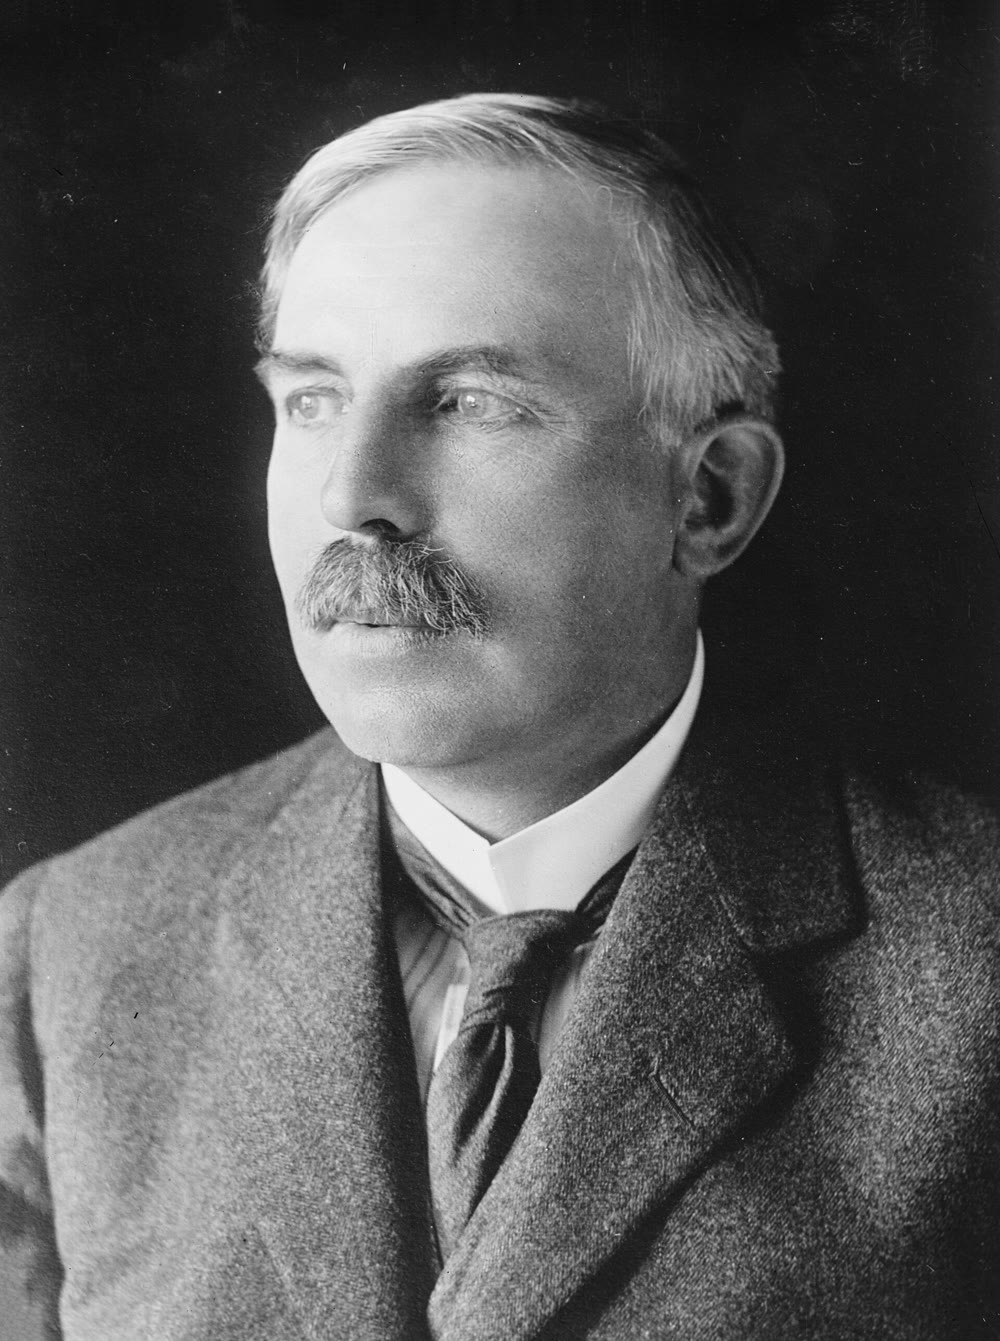
\includegraphics[width=\linewidth]{images/book1/rutherford.jpg}

{\small 欧内斯特·卢瑟福（1871--1937）。}
\end{minipage}\hfill
\begin{minipage}[b]{0.66\linewidth}\centering
\begin{tikzpicture}[font=\small]
  \fill[black!45] (0,-0.5) rectangle (0.9,0.5);
  \node[anchor=north, align=center] at (0.45,-0.55) {α 粒子源};
  \draw[->, thick, red!70!black] (0.9,0) -- (2.8,0);
  \fill[yellow!70!orange] (2.8,-1.6) rectangle (2.88,1.6);
  \node[anchor=north] at (2.84,-1.65) {金箔};
  \draw[omDef!40, line width=4pt] (5.6,-1.8) arc[start angle=-30, end angle=30, radius=3.6];
  \foreach \y in {-0.3,-0.1,0.1,0.3} \draw[->, red!70!black] (2.88,\y) -- (5.3,\y);
  \draw[->, red!70!black] (2.88,0.05) -- (5.0,1.15);
  \draw[->, red!70!black] (2.88,-0.05) -- (4.9,-1.3);
  \draw[->, red!70!black, thick] (2.8,0.02) .. controls (2.2,0.35) .. (1.6,0.95);
  \node[anchor=west, align=left, font=\footnotesize] at (6.25,0) {大多数 \\ 直线穿过};
  \node[anchor=south, align=center, font=\footnotesize] at (1.6,1.0) {极少数 \\ 被弹回};
\end{tikzpicture}

{\small 金箔实验：大多数粒子直线穿过；
少数粒子发生偏折，极少数从\omterm{def:g9:inside-the-atom:nucleus}{原子核}处弹回。}
\end{minipage}
\end{omfigure}

\section{练习}

\begin{exercise}[$\star$]\label{exo:g9:inside-the-atom:1}
说出\omterm{def:g9:inside-the-atom:nucleus}{原子核}中的粒子及核外粒子，
并写出它们所带电荷的正负号。
\end{exercise}

\begin{exercise}[$\star$]\label{exo:g9:inside-the-atom:2}
写出 \ce{^{16}_{8}O}、\ce{^{27}_{13}Al}
和 \ce{^{40}_{20}Ca} 中\omterm{def:g9:inside-the-atom:proton}{质子}、\omterm{def:g9:inside-the-atom:proton}{中子}和\omterm{def:g9:inside-the-atom:nucleus}{电子}的数目。
\end{exercise}

\begin{exercise}[$\star$]\label{exo:g9:inside-the-atom:3}
为什么\omterm{def:g7:atoms-and-molecules:atom}{原子}呈电中性？
\end{exercise}

\begin{exercise}[$\star$]\label{exo:g9:inside-the-atom:4}
某\omterm{def:g7:atoms-and-molecules:atom}{原子}有 26 个\omterm{def:g9:inside-the-atom:proton}{质子}和 30 个\omterm{def:g9:inside-the-atom:proton}{中子}，写出其核素符号（
\omterm{def:g9:inside-the-atom:element}{元素}为铁，\ce{Fe}）。
\end{exercise}

\begin{exercise}[$\star\star$]\label{exo:g9:inside-the-atom:5}
\ce{^{35}_{17}Cl} 和 \ce{^{37}_{17}Cl} 是否为同一种\omterm{def:g9:inside-the-atom:element}{元素}？它们
是否互为\omterm{def:g9:inside-the-atom:isotope}{同位素}？请说明理由。
\end{exercise}

\begin{exercise}[$\star\star$]\label{exo:g9:inside-the-atom:6}
\ce{^{14}_{6}C} 与 \ce{^{14}_{7}N} 是否互为\omterm{def:g9:inside-the-atom:isotope}{同位素}？请说明理由。
\end{exercise}

\begin{exercise}[$\star\star$]\label{exo:g9:inside-the-atom:7}
用科学记数法计算一个
\ce{^{56}_{26}Fe} \omterm{def:g7:atoms-and-molecules:atom}{原子}的近似质量。
\end{exercise}

\begin{exercise}[$\star\star$]\label{exo:g9:inside-the-atom:8}
在金箔实验中，为什么大多数粒子会
直线穿过金箔？
\end{exercise}

\begin{exercise}[$\star\star$]\label{exo:g9:inside-the-atom:9}
\omterm{def:g7:atoms-and-molecules:atom}{原子}的尺寸为 \qty{e-10}{m}，\omterm{def:g9:inside-the-atom:nucleus}{原子核}的尺寸为
\qty{e-15}{m}。\omterm{def:g9:inside-the-atom:nucleus}{原子核}比\omterm{def:g7:atoms-and-molecules:atom}{原子}小多少倍？用 10 的幂表示答案。
\end{exercise}

\begin{exercise}[$\star\star$]\label{exo:g9:inside-the-atom:10}
为什么同一\omterm{def:g9:inside-the-atom:element}{元素}的\omterm{def:g9:inside-the-atom:isotope}{同位素}具有相同的化学性质？
\end{exercise}

\begin{exercise}[$\star\star\star$]\label{exo:g9:inside-the-atom:11}
一个铁\omterm{def:g7:atoms-and-molecules:atom}{原子}有 26 个\omterm{def:g9:inside-the-atom:nucleus}{电子}。先计算这些\omterm{def:g9:inside-the-atom:nucleus}{电子}的总质量，
再计算它们占一个 \ce{^{56}_{26}Fe} \omterm{def:g7:atoms-and-molecules:atom}{原子}质量的比例（
用练习~7 中求得的质量）。
\end{exercise}

\begin{exercise}[$\star\star\star$]\label{exo:g9:inside-the-atom:12}
% ledger: iso:Cu63, iso:Cu65
天然铜中，\qty{69.15}{\percent} 为铜-63，\qty{30.85}{\percent}
为铜-65。在 10\,000 个铜\omterm{def:g7:atoms-and-molecules:atom}{原子}中，各\omterm{def:g9:inside-the-atom:isotope}{同位素}分别有多少个？
每个铜\omterm{def:g7:atoms-and-molecules:atom}{原子}的平均\omterm{def:g9:inside-the-atom:proton}{核子}数是多少？
\end{exercise}

\clearpage % keeps the heading with its problem box (it was stranded at a page foot)
\section{问题：称量氯}

\begin{problem}[{周末问题——氯的两种同位素，每个原子的质量，
以及氯原子的平均质量}]
\label{pb:g9:inside-the-atom:1}
% ledger: iso:Cl35, iso:Cl37, const:me, const:mp, const:mn
天然氯是两种\omterm{def:g9:inside-the-atom:isotope}{同位素}的\omterm{def:g6:pure-substances-and-mixtures:mixture}{混合物}，即氯-35 和
氯-37：在 1000 个氯\omterm{def:g7:atoms-and-molecules:atom}{原子}中，约 758 个为氯-35，
242 个为氯-37。取一个\omterm{def:g9:inside-the-atom:proton}{核子}的质量为 \qty{1.67e-27}{kg}，
一个\omterm{def:g9:inside-the-atom:nucleus}{电子}的质量为 \qty{9.11e-31}{kg}。氯的
\omterm{def:g9:inside-the-atom:atomic-number}{原子序数}为 17。

\medskip
\noindent\textbf{第一部分——两个\omterm{def:g9:inside-the-atom:nucleus}{原子核}。}
\begin{enumerate}
  \item 写出两种\omterm{def:g9:inside-the-atom:isotope}{同位素}的核素符号。
  \item 分别写出每种\omterm{def:g7:atoms-and-molecules:atom}{原子}的\omterm{def:g9:inside-the-atom:proton}{质子}数、\omterm{def:g9:inside-the-atom:proton}{中子}数和\omterm{def:g9:inside-the-atom:nucleus}{电子}数。
  \item 两者为什么都叫氯？它们为什么互为\omterm{def:g9:inside-the-atom:isotope}{同位素}？
  \item 氯-37 样品与钠的反应是否与
        氯-35 样品相同？请说明理由。
\end{enumerate}

\medskip
\noindent\textbf{第二部分——每个\omterm{def:g7:atoms-and-molecules:atom}{原子}的质量。}
\begin{enumerate}[resume]
  \item 计算一个氯-35 \omterm{def:g7:atoms-and-molecules:atom}{原子}的\omterm{def:g9:inside-the-atom:nucleus}{原子核}质量。
  \item 计算 17 个\omterm{def:g9:inside-the-atom:nucleus}{电子}的质量，并检验它与\omterm{def:g9:inside-the-atom:nucleus}{原子核}相比
        是否可以忽略不计。
  \item 计算一个氯-37 \omterm{def:g7:atoms-and-molecules:atom}{原子}的质量。
  \item 质量为 \qty{1}{g} 的氯-35 \omterm{def:g7:atoms-and-molecules:atom}{原子}有多少个？请用
        科学记数法表示结果。
\end{enumerate}

\medskip
\noindent\textbf{第三部分——平均\omterm{def:g7:atoms-and-molecules:atom}{原子}。}
\begin{enumerate}[resume]
  \item 氯-35 和氯-37 各占氯\omterm{def:g7:atoms-and-molecules:atom}{原子}的百分之几？
  \item 在 1000 个天然氯\omterm{def:g7:atoms-and-molecules:atom}{原子}中，计算氯-35 \omterm{def:g7:atoms-and-molecules:atom}{原子}和
        氯-37 \omterm{def:g7:atoms-and-molecules:atom}{原子}的总质量。
  \item 计算这 1000 个\omterm{def:g7:atoms-and-molecules:atom}{原子}的总质量。
  \item 由此推算一个氯\omterm{def:g7:atoms-and-molecules:atom}{原子}的平均质量。
\end{enumerate}
\end{problem}
